\documentclass[11pt]{article}
\usepackage[a4paper,margin=1in]{geometry}
\usepackage{amsmath,amssymb}
\usepackage{booktabs,longtable,array,calc,tabularx}
\usepackage{graphicx}
\usepackage[hyphens]{url}
\usepackage[colorlinks=true,linkcolor=black,urlcolor=blue,citecolor=blue]{hyperref}
\usepackage{caption}
\usepackage{placeins}
\usepackage{enumitem}
\setlength{\parskip}{0.45em}\setlength{\parindent}{0pt}
\setlength{\tabcolsep}{4pt}
\title{Supplementary information to: Does a one-pool water-balance model improve forecasts of Edwards Aquifer head? A scored test at J-17}
\author{Amin Abaee}
\date{October 16, 2026}
\begin{document}
\maketitle

\section*{Supplementary Information (v3)}

This supplement accompanies standalone E3 v25. S1 records the independent uncertainty replication; S2 documents where E3 SI v2 climate-window material is carried forward; S3 preserves the reproducibility manifest from v2. S4--S11 add the protocol, origin-set, fixed-window, uncertainty, threshold-indicator, Comal, pumpage, and climate details also inspected in Paper11 v67 SI S15--S22. These are diagnostic or post-freeze layers and do not alter the frozen retention rule.

\subsection{S1 Independent replication of the uncertainty
layer}\label{s1-independent-replication-of-the-uncertainty-layer}

An independent replication of this layer is archived with the
analysis record: the archived script
\texttt{campaign\_e3\_dm\_uncertainty.py}, a second Diebold--Mariano +
moving-block-bootstrap implementation --- HAC lag h − 1 with unweighted
truncation and population-variance scaling, block length h, 20,000
replications, seed 0, deterministic (byte-identical on re-execution) ---
reading the same archived per-origin forecast file. Its archived
output reproduces every load-bearing reading:
the M1 retention margin DM z = −0.86 with block CI {[}−1.22, +0.56{]} ft
(bootstrap p = 0.38); the M2m edge over persistence (p = 0.001); the h =
5 climatology win (p = 0.035). It also reports two rows the main table
does not carry --- the h = 1 climatology loss (+2.94 ft against
persistence, p = 0.046) and the M2 h = 5 loss (+12.4 ft, p \textless{}
0.001) --- both consistent with the readings above. The two
implementations use different seeds, block lengths, HAC weighting, and
variance conventions, and agree on every conclusion: the 0.39-ft AR(1)
retention margin is statistically indistinguishable from zero, the M2m
edge is the only one-year margin that separates from noise, and the
five-year climatology win survives.


\subsection{S2. Climate fixed-window record carried forward}

The climate fixed-window values reported as S2 in E3 SI v2 are retained in expanded form in S11. That section includes the recovery window as well as the drawdown, pre-permit, and critical-period windows, and preserves the recharge-target scores and the precipitation-oracle distinction. No scored climate-window result from v2 is dropped; S11 is the consolidated record for this version.

\subsection{S3 Reproducibility
package}\label{s3-reproducibility-package}

The numerical inputs and scores in the v25 main text and S1--S11 are
traceable to the analysis scripts and outputs archived at
https://github.com/MIKEAA2020/general-sustainability; checksums (md5,
first 8 hex) pin the release state. Execution is deterministic
throughout --- a fresh environment regenerated every archived result
file byte for byte. Two independent DM/bootstrap implementations (10,000
and 20,000 replications, different seeds, block lengths, HAC weighting,
and variance conventions) agree on every load-bearing conclusion; both
are archived, and the nClimDiv precipitation workbook is the sole raw
file not redistributed (provenance URL archived in the sources index;
scoring from the archived analysis panel does not require it).

{\def\LTcaptype{none} % do not increment counter
\begin{longtable}[]{@{}
  >{\raggedright\arraybackslash}p{(\linewidth - 6\tabcolsep) * \real{0.2500}}
  >{\raggedright\arraybackslash}p{(\linewidth - 6\tabcolsep) * \real{0.2500}}
  >{\raggedright\arraybackslash}p{(\linewidth - 6\tabcolsep) * \real{0.2500}}
  >{\raggedright\arraybackslash}p{(\linewidth - 6\tabcolsep) * \real{0.2500}}@{}}
\toprule\noalign{}
\begin{minipage}[b]{\linewidth}\raggedright
Script (repo path)
\end{minipage} & \begin{minipage}[b]{\linewidth}\raggedright
Role in the paper
\end{minipage} & \begin{minipage}[b]{\linewidth}\raggedright
md5
\end{minipage} & \begin{minipage}[b]{\linewidth}\raggedright
\end{minipage} \\
\midrule\noalign{}
\endhead
\bottomrule\noalign{}
\endlastfoot
\texttt{wave\_e\_edwards/src/build\_panel.py} & Builds the archived
twenty-column analysis panel (dataset of record) & \texttt{2cfd1649} &
results analysis panel \\
\texttt{wave\_e\_edwards/src/build\_climate.py} & Builds the climate
(Niño 3.4, precipitation) panel columns & \texttt{356af249} & climate
panel \\
\texttt{wave\_e\_edwards/src/run\_ladder.py} & J-17 model ladder
scoring, persistence and oracle diagnostics & \texttt{e01f29cd} &
results rolling\_forecasts.csv, window tables \\
\texttt{wave\_e\_edwards/src/e3\_audit\_uncertainty.py} & Main
post-freeze uncertainty layer: DM + Newey--West HAC + moving-block
bootstrap, 10,000 replications, seeded, deterministic &
\texttt{074ff015} &
wave\_e\_edwards/results/e3\_audit\_uncertainty.json \\
\texttt{batch\ 7\ (audits\ of\ agent\ arena\ 1\ paper\ rewrites)/campaign\_e3\_dm\_uncertainty.py}
& Independent replication of the same layer: NB = 20,000, seed 0,
byte-identical re-execution & \texttt{30963493} &
results/e3\_dm\_uncertainty.csv \\
\texttt{arena\_agent\_1/other\ documents/rerun\_campaigns/campaign\_e3\_pumpage\_scenarios.py}
& Pumpage counterfactual layer of Section 5.6 & \texttt{c3fe4fe3} &
scenario table outputs \\
\texttt{wave\_e\_edwards/src/make\_figures.py} & Generates the J-17 series, rolling-score, fixed-window, climate-pass, and Comal figures used in v25 main text and SI & \texttt{57c17e29} & \texttt{figs/edw\_fig1\_series.png}--\texttt{edw\_fig5\_fibre.png} \\
\end{longtable}
}


\subsection{S4. Protocol record and deviations}\label{si:edwprotocol}

The scoring protocols for the primary pass and climate pass were frozen and dated (2026-08-25) before the corresponding RMSE tables were computed, and are archived with the analysis code. This is a frozen computational protocol, not a prospective registration. The archived rule reads:

\begin{quote}\small
Let $\mathrm{RMSE}(\cdot)$ denote the primary rolling-origin RMSE at a fixed horizon $h$. A causal module $M$ is retained only if: (H1) $\mathrm{RMSE}(M) < \mathrm{RMSE}(\text{persist})$, i.e.\ it beats last-value persistence, and (H2) $\mathrm{RMSE}(M) < \mathrm{RMSE}(M_{\text{next-simpler causal}})$, i.e.\ it beats the next-simpler causal model. Retention is decided at $h=1$ on the point-RMSE comparison; no tie tolerance and no minimum margin is imposed. Diagnostic oracles are excluded from retention. The Comal series is excluded from retention. Retention is decided on the head series only; the service series is scored after that decision is frozen.
\end{quote}

The main text labels these hurdles H1 and H2. The archived rule uses the phrase ``causal module'' for the process-structured candidates; this is not a causal-identification claim. The primary score is RMSE of annual-mean J-17 in feet; secondary scores are mean absolute error and the Brier score of $\mathbf{1}\{\hat H<660\}$, interpreted only for origins at or after 2007 (S8). A sign-hit rate of $\Delta H$ was listed in an earlier design iteration and is struck: no value is reported for it and it is not part of any retention decision.

Three protocol elements sit outside the frozen rule and are recorded here as deviations, in one place.
\begin{enumerate}[leftmargin=2em]
\item \textbf{The M2m class clause.} M2m is listed and then declined on class grounds (main-text class discussion). The clause is in the frozen protocol document, but it is not in the retention rule; under the rule as written, M2m satisfies H1 and H2 at $h=1$ (12.28 against 13.23 and 12.84\,ft).
\item \textbf{The climate-rung comparator.} The frozen Pass-2 protocol states the climate question as whether a process-structured recharge forecast reduces primary RMSE on J-17 ``relative to persistence and relative to M1'', the retained M1. The comparator is read accordingly. Declaring the declined M2m as the rung's H2 comparator would be inconsistent with the frozen document and circular, since the gate would be a model the protocol had itself declined. The M2m margins are retained as a nested-baseline reading rather than as the gate. At $h=1$, M2\_Renso (12.82), M2\_Rprecip (12.80), and M2\_combo (12.71) are each below M1 (12.84) and persistence (13.23); M2\_Rar (13.25) is not. The archived scoring code first lists these three under the strict point rule, then class-demotes them as M2m-plus-intercept variants rather than additional head-forecast structure. Thus the v67 statement that the final ``none retained'' disposition is unchanged under either comparator is true only at the broader structural-decision level: with M1, three pass the point gate and are then demoted; with M2m, none clears the point comparison. It must not be read as three failures of the frozen M1/persistence point rule. The v67 discussion also cites the small, statistically indistinguishable margins and worse $h=5$ scores; the latter hold the one-step recharge forecast fixed and are not a multi-year climate test. No significance threshold or $h=5$ hurdle appears in the frozen point rule. E3 v25 therefore reports the three point-rule passes and the separate class-based disposition without retrofitting either as a new gate. The best margin's paired uncertainty analysis does not distinguish a climate gain from zero.
\item \textbf{The struck sign-hit score.} Direction-of-change accuracy for $\Delta H$ appeared in an earlier design iteration and was struck; the corresponding score is neither computed nor reported, and it does not enter any retention decision.
\end{enumerate}

Post-freeze objects, labelled as such: the climate-pass fixed-window scores (S11), the pumpage counterfactuals (S10), the Comal service-series scoring (S9), and the uncertainty layer (S7) together with its independent replication. None replaces or alters a frozen verdict.

\subsection{S5. Origin sets, windows and data processing}\label{si:edworigins}

\paragraph{Rolling origin} Minimum 15 training years; the first origin is 1948 and forecasts target years through 2023, giving $n=75$ origins at $h=1$ and $n=71$ at $h=5$. Every model in the rolling tables, including M2m and the climate variants, is scored on the identical origin sets. Early rolling origins with the 15-year floor give 14 transitions for a four-parameter fit, so the process-model family's rolling scores carry unstable early-window coefficients.

\paragraph{Fixed windows} (1) Drought-of-record drawdown: train 1934--1950 (16 transitions), test 1951--1956. (2) Drought-of-record recovery: train 1934--1956 (22), test 1957--1961. (3) Pre-permit wet interval: train 1980--1990 (10), test 1991--1995. (4) Critical-period era: train 1997--2014 (17), test 2015--2023.

\paragraph{Head series} Annual means use all available daily highs of TWDB well 6837203. Years with fewer than 240 observations would be dropped; no year falls below the floor (minimum $n=242$, 1939), so the rule never binds. 1935 ($n=258$) and 1939 ($n=242$) are retained as incomplete-coverage means; missing days are not interpolated; the published pre-continuous composite (Beverly Lodges extension) is used as issued; the complete estimation panel ends in 2023, whose values carry provisional TWDB status. The predictand is the calendar-year mean of daily \emph{highs}; a daily-mean convention would sit slightly lower and matters near the 660/618-ft lines, and the Authority's Stage~I rule is a 10-day mean, so the annual-mean indicator is a coarse proxy flagged where used. Stage~I at 660\,ft is a 2007 institutional rule and is not applied as if it existed in 1956.

\paragraph{Fluxes and climate} Recharge $R$ is USGS total San Antonio-area recharge ($10^3$ acre-ft\,yr$^{-1}$), Puente stream-loss method, constructed independently of J-17 (Umphres and Choi, 2025). Pumpage $P$ is well discharge from Edwards Aquifer Authority Table~1 (1934 onward). Total spring discharge is stored and not used as a driver; eastern-basin recharge was stored and not used. Climate predictors: September--November Ni\~no~3.4 (HadISST, anomaly relative to 1991--2020) and calendar-year precipitation in Texas climate divisions 06 and 07 (NCEI nClimDiv). December--February precipitation that includes January of $t+1$ is not used. The archived twenty-column analysis panel (\texttt{wave\_e\_edwards/data/annual\_panel.csv}) is the dataset of record for all scored analyses; the nClimDiv raw file is not redistributed (provenance URL archived), so its three columns rebuild from the provenance source rather than from the archive, while the two Ni\~no columns rebuild from the archived file to machine precision.

\paragraph{Information set} Information known at 31 December of year $t$ comprises $(H,R,P)$ through $t$, the September--November Ni\~no~3.4 anomaly of year $t$ and calendar-year precipitation of year $t$. A two-pool exchange module was specified and not fitted; no barrier or exchange term was fitted. Post-1997 pumpage no longer spikes with drought as in 1956 ($321\times10^3$ acre-ft from wells); that change is already in $P_t$, and a separate critical-period switch adds no degree of freedom beyond the pumpage series.

\FloatBarrier
\subsection{S6. Fixed windows}\label{si:edwfixed}

Table~\ref{tab:si_edwfixed} and Fig.~\ref{fig:si_edwwindows} give the fixed-window scores. They are diagnostic, not retention. On the drawdown window the bolded M2 is a continuing-drought artefact, not a forecasting merit: the last observed $R$ is already low, and the map trained on 1934--1950 has the wrong sign on pumpage ($\gamma=+0.021$), since pumping rose as the drought deepened and least squares aliases the human response into the state transition (simultaneity bias, compounded by the short window). That identification failure is why M2 ``beats'' the oracle there. The train-mean baseline is the best non-oracle forecast on the recovery window (14.07\,ft) and the critical-period era (14.77\,ft), consistent with its rolling five-year win; the residual-persistence rungs M3/M4 track M2 on the drawdown (18.12/18.23 against 18.11\,ft); M4 is the best process-structured model on the pre-permit wet window (15.26\,ft); and the process-model family performs poorly on the recovery and critical-period windows.

The recovery window is also where the $[610,710]$ clip binds on forecast paths: the M2 trajectory with persisted $(R,P)=(43.7,321.1)$ runs $617.1\to611.6\to606.8\to605.3\to605.3$\,ft, reaching the 610-ft floor from 1959 onward. The clip never binds on the observed record (annual means 623--692\,ft); it binds only on these persisted-drought forecast paths, and it is doing work exactly there. The audit script recomputes both fixed-window M2 RMSEs (18.11 and 55.32\,ft) exactly from the archived panel. The 1957--61 recovery is a recharge pulse ($R_{1956}=43.7$, $R_{1957}=1142.6\times10^3$ acre-ft): persistence stays at the 1956 floor, M2 persists drought recharge and falls further, the oracle, given the 1957 flood year, tracks the rise. Recoveries on this specification are recharge events, not autonomous mean reversion, although the training mean (mean reversion) scores 14.07\,ft, second only to the oracle, in this institutionally bounded, rapidly recharged system.

\begin{table}[!htb]
\centering\small
\caption{J-17 fixed-window RMSE (ft). Bold marks the lowest RMSE of the window including the diagnostic oracle.}
\label{tab:si_edwfixed}
\begin{tabular}{@{}lrrrrrrrr@{}}
\toprule
Window & persist & mean & M1 & M2 & M2m & M3 & M4 & oracle \\
\midrule
Drawdown 1951--56 & 23.75 & 35.19 & 30.94 & \textbf{18.11} & 27.44 & 18.12 & 18.23 & 19.69 \\
Recovery 1957--61 & 43.62 & 14.07 & 56.24 & 55.32 & 37.74 & 55.28 & 55.12 & \textbf{12.26} \\
Pre-permit wet 1991--95 & 30.13 & 18.24 & 20.02 & 16.67 & 23.47 & 16.41 & 15.26 & \textbf{7.18} \\
Critical-period era 2015--23 & 27.41 & 14.77 & 15.62 & 23.37 & 14.79 & 22.84 & 22.17 & \textbf{8.70} \\
\bottomrule
\end{tabular}
\end{table}

\begin{figure}[!htb]
\centering
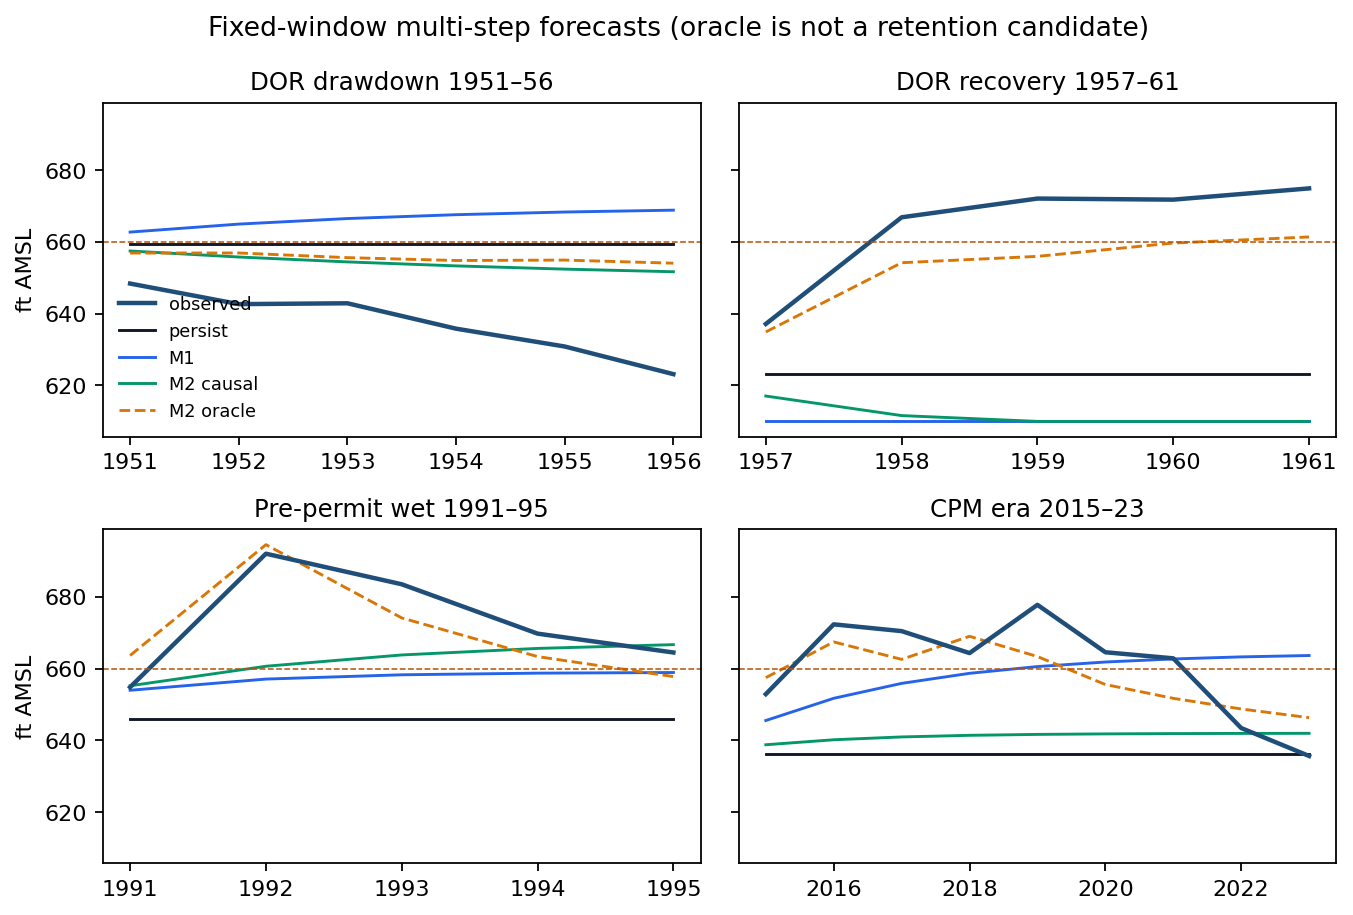
\includegraphics[width=\textwidth]{figs/edw_fig2_windows}
\caption{J-17 multi-step forecasts from the end of each training window. The oracle (dashed) is diagnostic and uses realized future $R,P$.}
\label{fig:si_edwwindows}
\end{figure}

\FloatBarrier
\subsection{S7. Uncertainty layer: two implementations}\label{si:edwuncertainty}

The post-freeze uncertainty layer (\texttt{e3\_audit\_uncertainty.py}; seed 20260905) attaches Diebold--Mariano tests (Newey--West HAC, lag $h-1$) and moving-block bootstrap intervals (block length 8, 10\,000 replications) to every load-bearing margin, computed from the archived per-origin forecast files; the main-text uncertainty summary reports its load-bearing readings. An independent replication (\texttt{campaign\_e3\_dm\_uncertainty.py}, archived with its output \texttt{e3\_dm\_uncertainty.csv}) is a second implementation reading the same archived per-origin forecast file: HAC lag $h-1$ with unweighted truncation and population-variance scaling, block length $h$, 20\,000 replications, seed 0, deterministic (byte-identical on re-execution). Its verified output reproduces every load-bearing reading: the M1 retention margin has DM $z=-0.86$ with block interval $[-1.22,+0.56]$\,ft (bootstrap $p=0.38$); the M2m edge over persistence has $p=0.001$; the $h=5$ climatology win has $p=0.035$. It also registers two rows the main table does not carry, the $h=1$ climatology loss ($+2.94$\,ft against persistence, $p=0.046$) and the M2 $h=5$ loss ($+12.4$\,ft, $p<0.001$), both consistent with the readings above. The two implementations use different seeds, block lengths, HAC weighting and variance conventions, and agree on every conclusion: the 0.39-ft AR(1) retention margin is statistically indistinguishable from zero, the M2m edge is the only one-year margin that separates from noise, and the five-year climatology win survives.

\subsection{S8. Threshold indicator scores on the post-2007 origins}\label{si:edwbrier}

The second secondary score is scoped to the post-2007 origins, where the 660-ft Stage~I rule is in force. On those origins ($n=16$ at $h=1$) the committed records give 660-ft Brier scores of 0.31 (persistence), 0.25 (M1), 0.25 (M2m), 0.19 (oracle), with the one-year RMSE ranking unchanged (persistence 13.09, M1 12.16, M2m 12.18, M2 13.31, oracle 8.03\,ft); at $h=5$ ($n=12$) the M1--persistence ordering reverses on the subsample (17.16 against 25.10\,ft) and the training mean scores 16.41\,ft, reported without changing the one-year retention statement. For deterministic 0/1 forecasts the Brier score is a misclassification rate of a coarse annual-mean proxy for the Authority's 10-day rule on a small subsample; the full record is archived as \texttt{wave\_e\_edwards/results/rolling\_modern\_2007.csv}.

\FloatBarrier
\subsection{S9. The service series after the retention freeze}\label{si:edwcomal}

The map $Q=c_0+c_1H$ fitted on 1934--1950 ($c_0=-2876$, $c_1=4.77$) is a linear channel of the same state indexed by J-17; the full-sample contemporaneous correlation is $r=0.986$ (Fig.~\ref{fig:si_edwfibre}). The channel fails in the drought tail, and the direction matters: at the 1956 annual mean (623.15\,ft) it reads $\approx97$\,cfs against an observed $\approx32$\,cfs annual mean, so it predicts non-cessation, and its zero-discharge level ($2876/4.77\approx602.9$\,ft) lies below every observed head (daily minimum 612.5\,ft), so the map never predicts cessation where cessation occurred. Near-linear at ordinary heads, the channel fails at cessation exactly where management cares. One-year Comal RMSE (cfs), scoring the same ladder directly on the Comal series over the same rolling origins ($n=75$): persist 71.9, M1 69.0, M2m 68.7, M2 74.8, M3 73.8, M4 73.4, train-mean 89.7, oracle 45.3; the ordering is broadly consistent with the strong near-linear association, but it is not an algebraic identity. The service series does not change retention, and it cannot: Comal is an independent measurement (a USGS spring gauge, not used to construct J-17) but not an independent information source.

\begin{figure}[!htb]
\centering
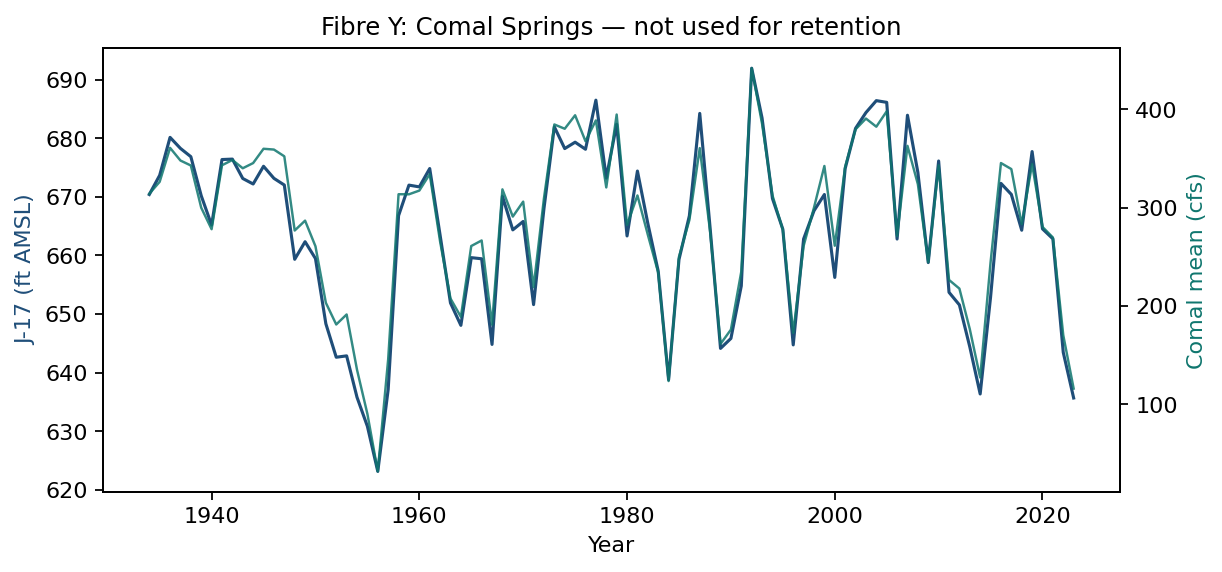
\includegraphics[width=0.85\textwidth]{figs/edw_fig5_fibre}
\caption{Comal annual mean against J-17. Contemporaneous $r=0.986$. The service series is a measured rating curve of the same state.}
\label{fig:si_edwfibre}
\end{figure}

\FloatBarrier
\subsection{S10. Pumpage counterfactuals}\label{si:edwpumpage}

A declared scenario layer passes counterfactual pumpage paths through the pre-permit affine map (train 1980--1990, the ladder's window~3; the short-window identification caveat applies to the map itself), from the observed 1990 head (645.8\,ft) over 1991--2023 with the actual recharge sequence (Table~\ref{tab:si_pumpage}). The scenarios are counterfactual simulations of the fitted map, not forecasts, and carry no retention implication. Four readings follow. First, pumpage is a secondary lever in this map: the full spread of counterfactual policies spans 630.9--646.8\,ft at 2023, and the map's own RMSE against the observed record (7.2--14.2\,ft) is of the same order as the policy spread, so the 5-ft effects are within model error and are not policy estimates. Second, the 20\%-cut path is the closest to the observed record of the four scenarios (7.19 against 8.56\,ft), an artefact of the map running high on this window (the actual-pumpage path ends 5.9\,ft above the observed 2023 head of 635.7\,ft), not evidence that the Authority's pumpage was near-optimal. Third, the direction is right and the magnitude modest: the 20\% cut raises the simulated 2023 head by 5.2\,ft relative to the actual-pumpage path. Fourth, the recharge coefficient dominates the map through its range, not its magnitude: a $1000\times10^3$ acre-ft recharge difference moves the head by roughly 17.5\,ft at the pre-permit coefficient ($\hat\beta\approx0.0175$; the pumpage coefficient on that train is $-0.031$\,ft per $10^3$ acre-ft, larger per unit but acting on a range of $\sim$300--540 against recharge's 44--2\,486), and $\gamma$ is an ordinary-least-squares association the paper itself diagnoses as simultaneity-contaminated (S6), not a policy lever. The full-sample coefficients $(\hat\beta,\hat\gamma)=(0.017,-0.026)$ differ from the pre-permit window's because the windows differ.

\begin{table}[!htb]
\centering\small
\caption{Pumpage counterfactuals, 1991--2023 (fitted pre-permit map; actual recharge). Pumpage: 1991--2023 mean in $10^3$ acre-ft\,yr$^{-1}$; heads, minimum head over the path and RMSE against the observed record in ft. The observed 2023 head is 635.7\,ft.}
\label{tab:si_pumpage}
\begin{tabular}{@{}lrrrr@{}}
\toprule
Scenario & pumpage & head 2023 & min.\ head & RMSE \\
\midrule
actual pumpage & 382.1 & 641.6 & 640.2 & 8.56 \\
pumpage frozen at 1990 & 489.4 & 630.9 & 630.5 & 14.22 \\
pre-permit mean pumpage & 469.8 & 632.4 & 632.0 & 13.02 \\
20\% pumpage cut & 305.7 & 646.8 & 645.5 & \textbf{7.19} \\
\bottomrule
\end{tabular}
\end{table}

\FloatBarrier
\subsection{S11. Climate-informed recharge: fixed windows, the recharge target, and the Uvalde note}\label{si:edwclimate}

Fig.~\ref{fig:si_edwpass2} shows the rolling climate-pass scores; the corresponding summary is in the main-text climate table. Same-year corr($R$, precipitation) $=0.78$, which is why the precipitation oracle reduces head RMSE to 10.56\,ft; it remains worse than the full $(R,P)$ oracle (7.55\,ft) because the linear rain map misses 1957-scale extremes. On the 1957--61 recovery no climate-informed module has lower RMSE than persistence (persist 43.6\,ft; best process-model variant 48.8\,ft; precipitation oracle 33.7\,ft); September--November 1956 is La Ni\~na ($-0.92$) and does not announce $R_{1957}=1143$. The remaining fixed windows complete the record: drawdown 1951--56, M2\_Renso 24.30, M2\_Rprecip 28.67, M2\_combo 24.70, M2\_Rar 31.38, precipitation oracle 18.16\,ft; pre-permit wet 1991--95, M2\_Rprecip 22.03, M2\_Renso 23.03, M2\_Rar 23.94, M2\_combo 25.71, oracle 10.98\,ft; critical-period era 2015--23, M2\_Rprecip 14.52, M2\_Rar 14.67, M2\_Renso 16.01, M2\_combo 16.57, oracle 9.75\,ft; on this one window the two climate-informed modules M2\_Rprecip and M2\_Rar edge past M1 by about one foot (14.52 and 14.67 against 15.62\,ft). On the recharge target itself the fixed-window scores are an order of magnitude coarser on every window (climate modules 199--937; precipitation oracle 80.7--487, against the $556\times10^3$ acre-ft climatology scale of the rolling record), so the marginal head advantage is a window-specific result, not a recharge forecast. Additional climate indices (PDO, AMO) were not run; they would enter through the same one-step recharge forecast and cannot alter the timing result. A mid-year operational forecast would require a new target-aligned evaluation protocol.

\begin{figure}[!htb]
\centering
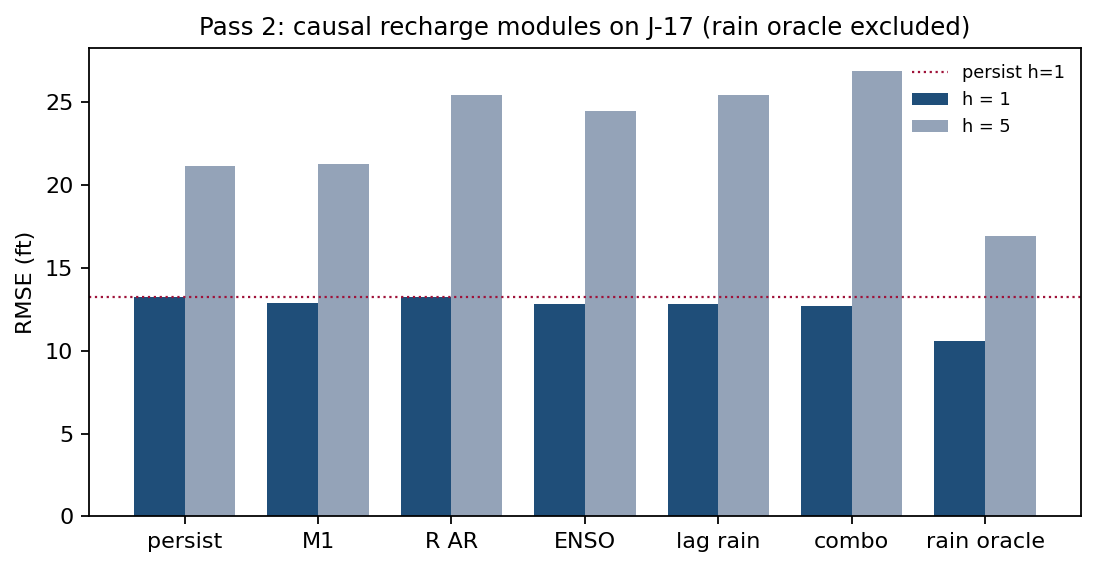
\includegraphics[width=0.85\textwidth]{figs/edw_fig4_pass2}
\caption{Rolling RMSE on J-17 for climate-informed recharge. The precipitation oracle uses year $t+h$ precipitation and cannot be retained.}
\label{fig:si_edwpass2}
\end{figure}

\paragraph{The Uvalde note} An exploratory port of the ladder to the separately regulated Uvalde Pool of the same aquifer (index well J-27; annual head lag-one autocorrelation 0.84) finds the AR(1) losing to persistence by 0.13\,ft at $h=1$, an exploratory observation only; it does not establish that the AR(1) margin must shrink in other pools. A single additional pool is a direction, not a test; no Uvalde result enters any retention verdict, the two records are not pooled, and the comparison is not offered as a test of anything claimed in the main text.

\end{document}
